\chapter{Problema 4}

\section{Minimal Coverage}

Dados segmentos de una l�nea (en el eje X) con coordenadas [$L_i$,$R_i$]. Se debe elegir la minima cantidad de estos segmentos, tales que cubran completamente el segmento [$0$,$M$].

\textbf{Input:}

El input esta dividido en varias partes:

La primera l�nea, consiste en un n�mero e indica la cantidad de casos de test, seguido de una l�nea en blanco.

Luego sigue el test, que consiste en un n�mero, que identifica el segmento [$0$,$M$] (donde $1<= M <= 5000$), seguido de pares $L_i$ $R_i$ que identifican segmentos ($|L_i|$, $|R_i|$ $<=50000$, e $i <= 100000$), cada uno separados por una linea. Cada test termina con el par $0$ $0$.

\textbf{Output:}

Para cada caso de test, la primera l�nea indica el m�nimo numero de segmentos que pueden cubrir el segmento [$0$,$M$]. En las l�neas siguientes, las coordenadas de los segmentos, ordenados por su coordenada izquierda ($L_i$), con el mismo formato que en el input. El par $0$ $0$ no debe ser mostrado.

Si [$0$,$M$] no puede ser cubierto, se debe devolver 0.

Cada resultado entre tests, debe estar separado por una l�nea en blanco.

\textbf{Url:}

\href{http://uva.onlinejudge.org/index.php?option=com\_onlinejudge\&Itemid=8\&category=12\&page=show\_problem\&problem=961}{Problema de minimal coverage}

\subsection{Soluci�n}

Para llegar a la soluci�n de este problema, se tuvo como idea de resoluci�n una t�cnica golosa, donde en cada paso se decide cuales de las opciones que se tienen disponibles en ese paso, garantizan un resultado �ptimo.

Dicha idea consiste b�sicamente, en ir tomando los intervalos que cubran mas a la derecha posible desde el intervalo cubierto hasta el momento y luego, una vez encontrado dicho intervalo, actualizar la zona cubierta hasta ese paso. Para hacer esto, como primera medida, se ordenan los intervalos recibidos como entrada del problema, de menor a mayor, por su primera coordenada. Con esta medida se pueden ir recorriendo en orden los intervalos de entrada y escoger aquel que nos pueda ayudar a dar un soluci�n optima.

A continuaci�n se describir�n los pasos mas importantes de la soluci�n para que la idea quede mejor explicada.

\begin{enumerate}
\item Paso 1: En este paso, se ordenan los intervalos recibidos como entrada del problema y se los ordena de menor a mayor por su primera componente. Esto se hace para facilitar la b�squeda del mejor intervalo en cada paso.
\item Paso 2: Utilizando la lista de pares ordenados del punto anterior, lo que se hace aqui, es recorrer cada par (intervalo) de forma tal de seleccionar aquel que tenga su segunda coordenada mas grande y que comience dentro del intervalo cubierto hasta el momento (es decir que su primera coordenada sea menor a cierto valor, que en principio es 0, ya que no se ha cubierto nada a�n).
\item Paso 3: Una vez obtenido el intervalo del paso 2, se actualiza el valor que representa lo cubierto hasta el momento, cambi�ndolo por la segunda coordenada del intervalo obtenido.
\end{enumerate}

A continuaci�n se mostrar� como el m�todo encuentra la soluci�n para un ejemplo, en donde se ingresan los intervalos $a = (-1,0)$, $b = (1,3)$, $c = (2,3)$, $d = (0,2)$ y donde el intervalo a cubrir es el $(0,3)$. 


\begin{figure}[H]
\centering
\subfigure[intervalos en el orden en que fueron ingresados.]{
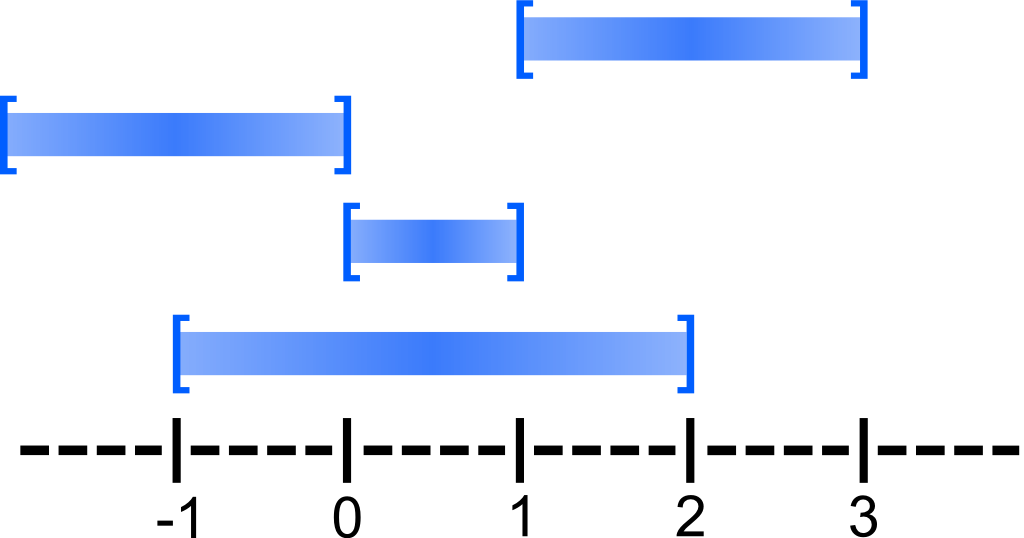
\includegraphics[scale=0.5]{./graficos/ej4/ej4_1_0.png} }\hspace{0.5in} 
\subfigure[intervalos una vez ordenados.]{
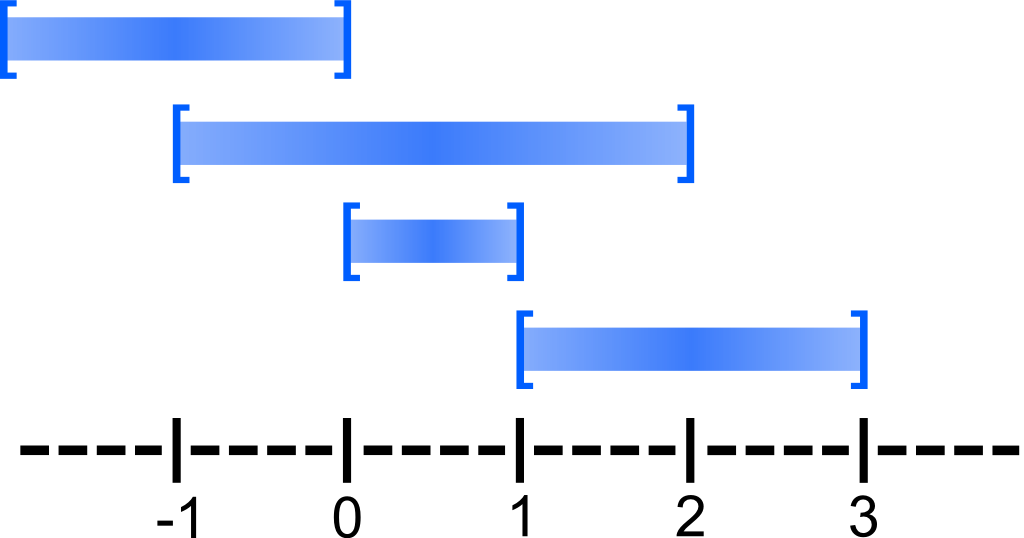
\includegraphics[scale=0.5]{./graficos/ej4/ej4_1_1.png}}\hspace{0.5in} 
\subfigure[seleccionar los intervalos que tengan alguna coordenada en el intervalo actual $[0,0]$]{
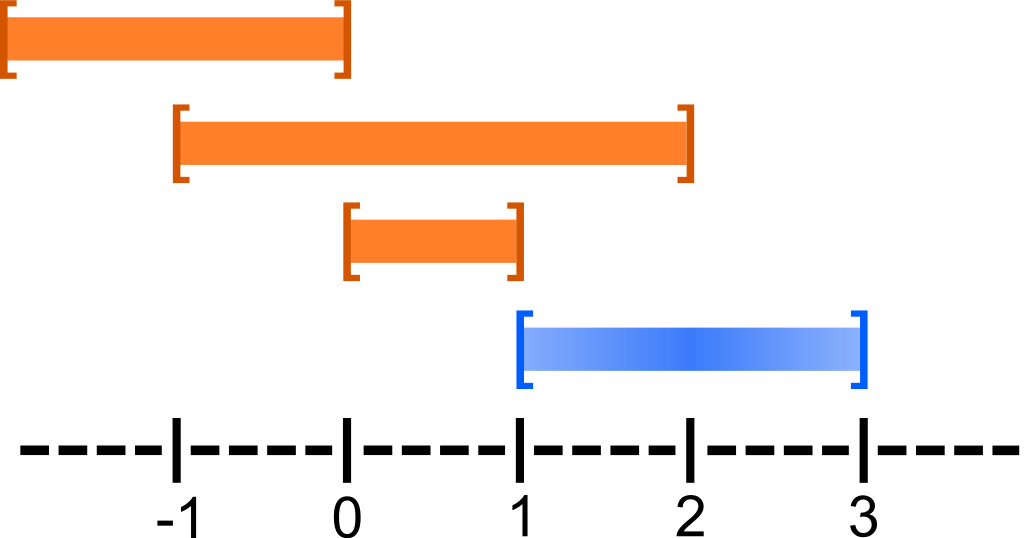
\includegraphics[scale=0.5]{./graficos/ej4/ej4_1_2.png}}\hspace{0.5in} 
\subfigure[se selecciona el que tiene la segunda coordenada mayor (intervalo d), se lo agrega como soluci�n, y se actualiza el itervalo actual a $[0,2]$]{
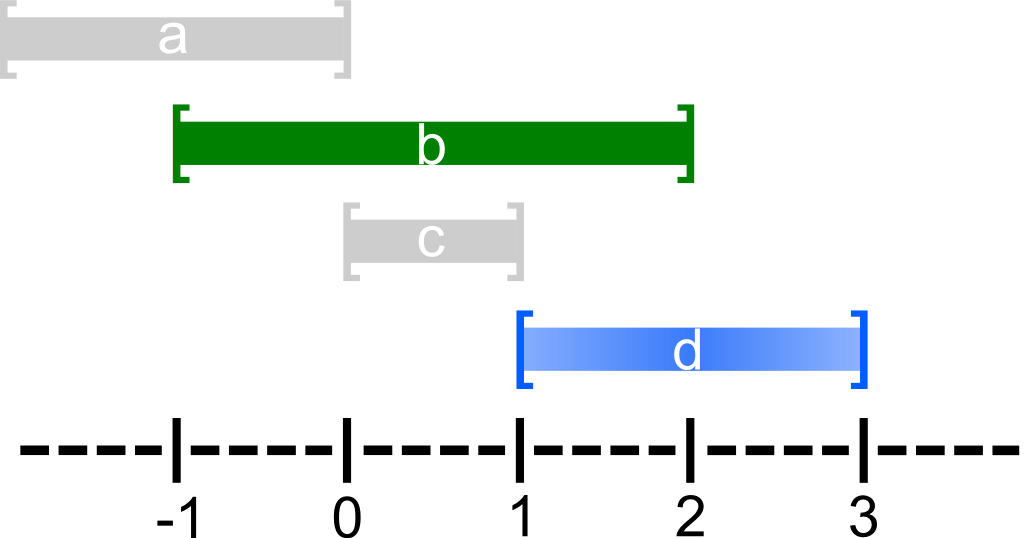
\includegraphics[scale=0.5]{./graficos/ej4/ej4_1_3.png}} \hspace{0.5in} 
\subfigure[se seleccionan los intervalos siguientes y que tengan alguna coordenada dentro del intervalo actual $[0,2]$]{
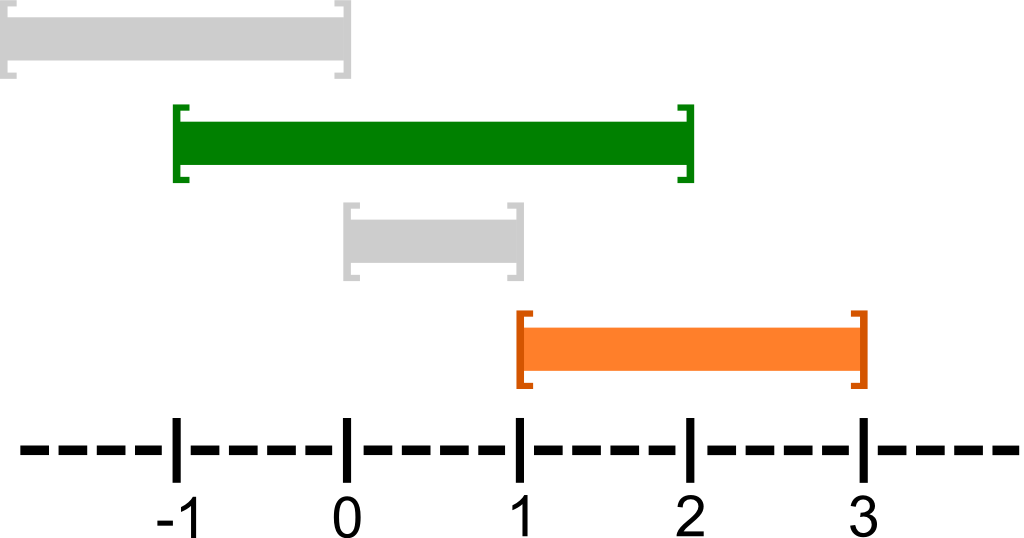
\includegraphics[scale=0.5]{./graficos/ej4/ej4_1_4.png} }\hspace{0.5in} 
\subfigure[se toma el de mayor segunda coordenada(intervalo b), se agrega como soluci�n y se actualiza el intervalo actual a $(0,3)$]{
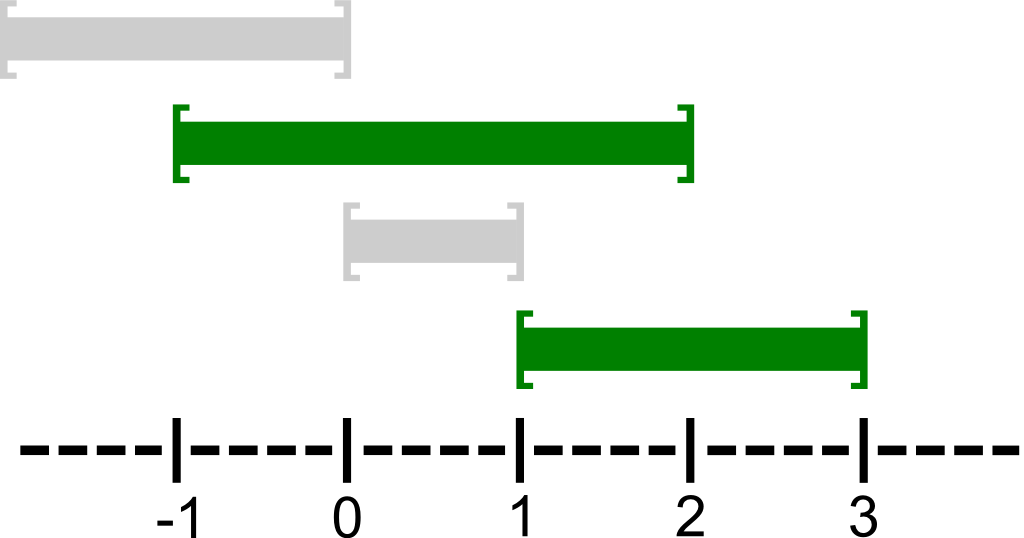
\includegraphics[scale=0.5]{./graficos/ej4/ej4_1_5.png}}
\caption{Pasos hasta hallar la soluci�n}
\setcounter{subfigure}{0}
\end{figure}

\subsection{Por qu� esta soluci�n?}

En cuanto al criterio de orden entre intervalos al momento de ordenarlos, elegimos que sea por su primera coordenada, pues esto nos permite avanzar (es decir, iterativamente agrandar el intervalo cubierto para llegar a la soluci�n) linealmente en el intervalo [0,M], lo que no es posible si el orden fuese por segunda coordenada. De usar un criterio de ordenamiento como este segundo, ser�a conveniente avanzar en el intervalo [0,M] desde fin a principio.

Ordenar los intervalos es escencialmente innecesario para el problema, pues para construir una soluci�n se podr�a recorrer siempre todos los intervalos y avanzar en [0,M] elegiendo seg�n el criterio del paso 2 del algoritmo. Sin embargo ordenar los intervalos nos asegura una mejor complejidad en peor caso.

El paso 2 nos asegura que no elegiremos intervalos de m�s y que el algoritmo siempre avanza y nunca vuelve en el intervalo ya cubierto. Al considerar aquellos pares que tengan su primera coordenada dentro del intervalo ya cubierto evitamos dejar \"huecos\" en el desarrollo de la soluci�n para no volver entre los intervalos ya vistos. Al elegir entre ellos aquel que tenga su mayor segunda coordenada logramos avanzar lo m�ximo posible en cada iteraci�n, sin perder soluciones. Veamoslo con un ejemplo:


El paso 3 nos asegura que el algoritmo termina, y que lo hace al cubrir el intervalo [0,M] o al encontrar un hueco dentro del mismo con los intervalos dados.

\subsection{C�lculo de complejidad}

\begin{algorithm}[H]
\caption{Calcula el step ladder de largo m�ximo}
\label{alg:algoritmo1b}
\begin{algorithmic}[1]
\PARAMS{cantidad de palabras}
\STATE inicializar los maximos step ladders de cada palabra en 1
\STATE inicializar maxLadder = 1
\FOR{cada palabra P}
	\STATE \COMMENT{borrado de letras}
	\STATE borrar de a un caracter por vez de P y buscar esta nueva palabra en las palabras anteriores a P
	\STATE si se encuentra actualizar el max step ladder de P
	\STATE \COMMENT{reemplazo de letras}
	\STATE reemplazar las letras de P de a una por vez por las letra del abecedario desde `a� hasta la letra a cambiar, formando $P'$
	\STATE buscar $P'$ en las palabras anteriores a P
	\STATE si se encuentra actualizar el max step ladder de P
	\STATE \COMMENT{agregado de letras}
	\STATE agregar letras de a una por vez en cada posicion de P formando $P'$
	\STATE buscar $P'$ en las palabras anteriores a P
	\STATE si se encuentra actualizar el max step ladder de P
	\STATE actualizar maxLadder
\ENDFOR
\RETURN maxLadder
\end{algorithmic}
\end{algorithm}
